%!TEX root = ../MasterThesis.tex

\section{Computer-Supported Cooperative Work}
\label{sec:cscw}

This section gives a short introduction to the theoretical foundations of \gls{CSCW} systems. It starts with an overview of the research field itself, followed by a description of the types of \gls{CSCW} systems available. After that it explains the concept of shared information spaces in detail.

\subsection{Fundamental aspects}
\label{sec:cscw_definition}

\gls{CSCW} is ``a \emph{generic} term which combines the understanding of the way people work in groups with the enabling technologies of computer networking, and associated hardware, software, services and techniques'' \citep[pg. 92]{borghoff2000computer}. It is part of the research field of \emph{Cooperation Systems}, which emerged during the early 1980s with the understanding that a multi-disciplinary approach for designing \gls{IT} systems is needed for the success of such systems. As such the research field looks into the usage of applications to support group work in an organizational setting, the effects of such a system on individual users, as well as how the applications have to be adapted for the context of the group. Therefore the studies of Cooperation Systems are consisting of a \emph{social} part as well as a \emph{technical} part, and are looking into the interrelationship between them for certain aspects of work in general, and explicitly for communication and cooperation in a team \citep{Grudin1994}. \\

These systems are generally focussed on the concept of human-centered computing that wants to establish technology and work methods to improve processes and results of the work, while also improving the human conditions at work. A ``work system'' in such a sense describes the process of human work that consists of goal-directed activities in a \emph{professional} context. As more work has been moved to information workers another important aspect of such a system is the human cognition, which results in a need of taking human behavior as well as individual goals and knowledge into consideration. Therefore ``work systems'' focus on activities that is done by a group of people, a team, an organisation or a society, and includes social factors like knowledge, goals, tasks and work of individuals or subgroups. These ``work systems'' are getting more and more complex as the problems human have to deal with are getting more difficult; in terms of their dynamic, nonlinear, interactive and simultaneous nature. Therefore humans have to continually adapt, take over different roles, and are engaged in various activities, which include management of the technologies used and handle the issues they introduce \citep{Hoffmann2009}. \\

That said a ``work system'' in this sense has two possible outcomes: the products and services created together by humans and/or machines and the sociological and psychological consequences as a result of being part of the process. The objective of a \emph{sociotechnical system} is to optimise both outcomes (see Figure~\ref{fig:images_sociotechnical_system}). To conclude \emph{sociotechnical} refers to the interrelatedness of social and technical aspects of an organization. The sociotechnical theory is founded on two main principles \citep{Koch2008}: \@

\begin{itemize}
  \item The interaction of social and technical factors creates the conditions for successful organizational performance. This interaction consists partly of linear ``cause and effect'' relationships and partly from ``non-linear'', often unpredictable relationships. Whether designed or not, both types of interaction occur when socio and technical elements are put to work.
  \item An optimization of each aspect alone (socio or technical) tends to increase not only the quantity of unpredictable relationships, but those relationships are injurious to the system's performance.
\end{itemize}

\begin{figure}[H]
 \centering
 %\includesvg[width=0.8\columnwidth, svgpath = images/]{cscw_time_place_matrix}
 \includegraphics[width=0.9\columnwidth]{images/sociotechnical_system.png}
 \caption[A sociotechnical work system]{A sociotechnical work system \citep{xx}}
\label{fig:images_sociotechnical_system}
\end{figure}

% section cscw_defintion (end)

\subsection{Classification of \gls{CSCW} systems}
\label{sec:cscw_types}

In a distributed team environment the style of communication could be \emph{synchronous} or \emph{asynchronous} depending on the dimension of time. If the communication takes place at the same time the communication is synchronous, otherwise asynchronous. Another aspect that needs to be taken into account is the place, which leads to the quadrant shown in Figure~\ref{fig:images_cscw_time_place_matrix}. \@

\begin{figure}[H]
 \centering
 %\includesvg[width=0.8\columnwidth, svgpath = images/]{cscw_time_place_matrix}
 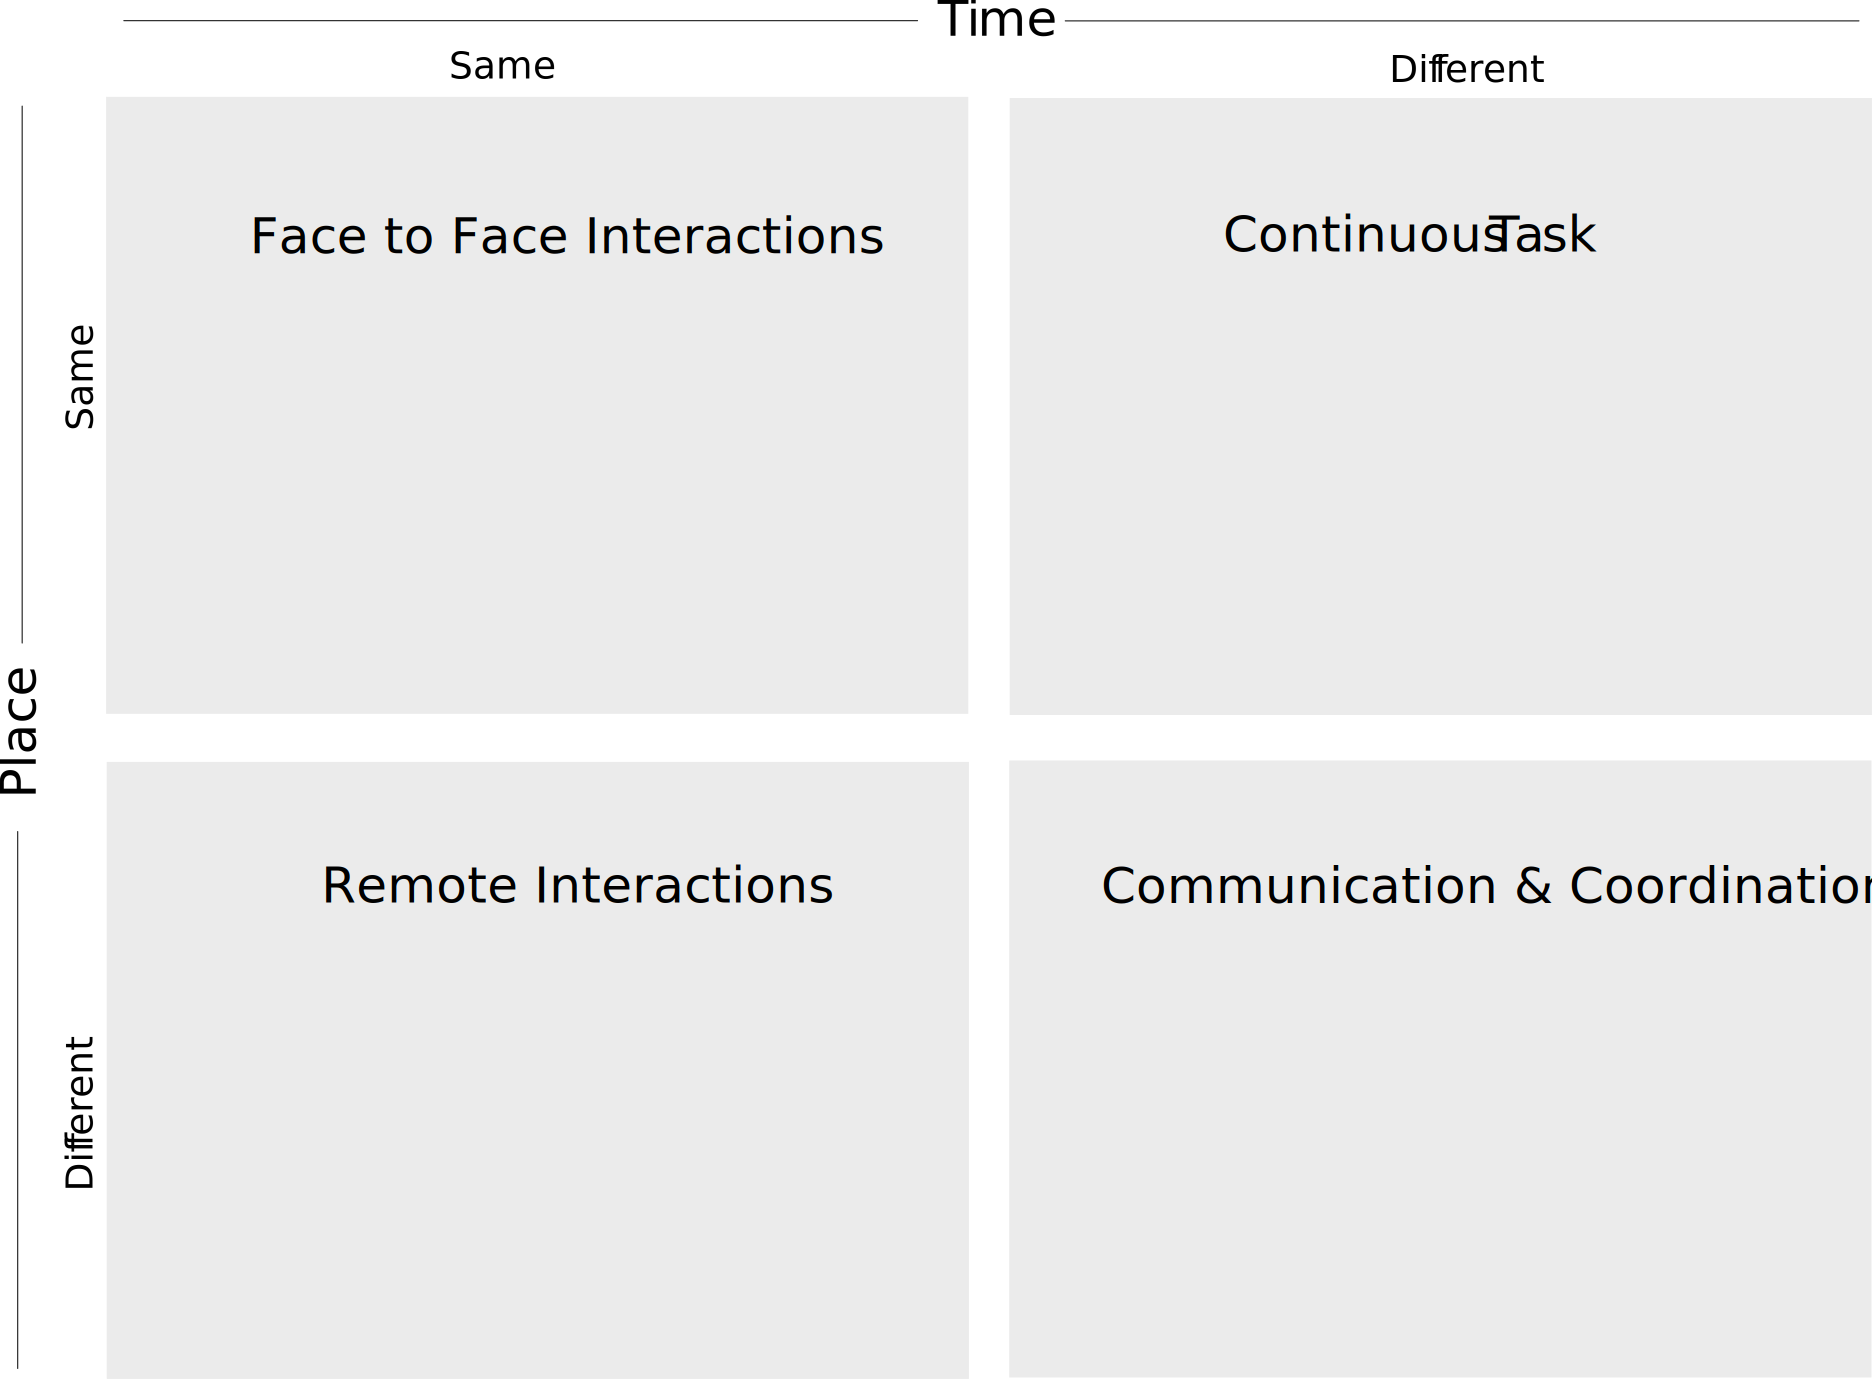
\includegraphics[width=0.8\columnwidth]{images/cscw_time_place_matrix.pdf}
 \caption[CSCW Place/Time Matrix]{\gls{CSCW} Place/Time Matrix \citep{xx}}
\label{fig:images_cscw_time_place_matrix}
\end{figure}

Additionally it is possible to group the CSCW systems based on the 3C model into \citep{Koch2008}:

\begin{itemize}
  \item \textbf{communication:} a two way exchange of information between different parties,
  \item \textbf{coordination:} management of shared resources such as meeting rooms, network printers, file shares, \ldots,
  \item \textbf{collaboration:} members of a group work together in a shared environment to reach a goal.
\end{itemize}

\begin{figure}[H]
 \centering
 %\includesvg[width=0.5\columnwidth, svgpath = images/]{cscw_time_place_matrix}
 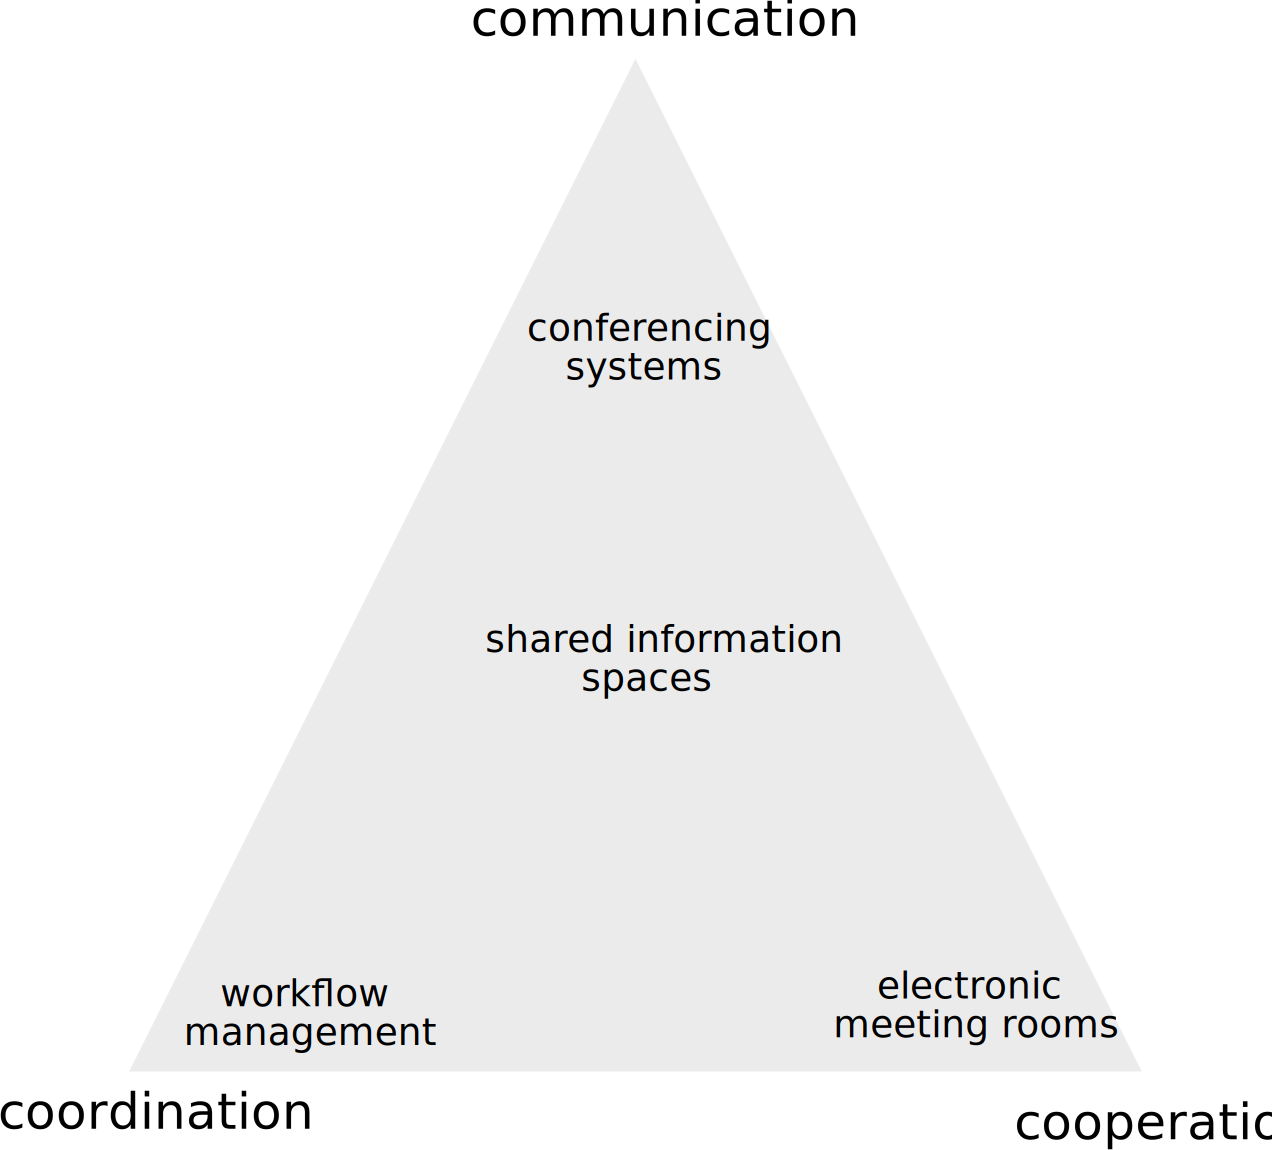
\includegraphics[width=0.8\columnwidth]{images/3C-model.pdf}
 \caption[The 3C Model]{The 3C Model \citep{Koch2008}}
\label{fig:images_cscw_3C_model}
\end{figure}

Typical examples might be (see also Figure~\ref{fig:images_cscw_3C_model}):

\begin{itemize}
  \item \textbf{group editors:} allows collaborated work on some kind of shared document or artefact; can face issues to keep the document in sync and setting up proper user roles and access rights,
  \item \textbf{shared information spaces:} also known as team rooms, cloud storage services, or document management systems that allow participants to access information at any place any time as well as to share information with others,
  \item \textbf{whiteboards:} allow multiple participants to work on a shared workspace and show the current and past activities of each of them; best used for ad-hoc brainstorming or idea generation.
\end{itemize}

% section cscw_types (end)

\subsection{Shared Information Spaces}
\label{sec:cscw_shared_spaces}

% section cscw_shared_spaces (end)

% section cscw (end)
